\chapter{String manipulation}
	\label{ch:strings}

	This chapter explains:
	\begin{itemize}
    \item the string facilities you have seen so far;
    \item the main methods and properties of the \keyword{String} class.
	\end{itemize}


	\section{Introduction}
		Strings of characters are very important in software. All programming languages have facilities for primitive character manipulation, but VB has a particularly useful collection of methods. In this chapter, we will bring together the string features we have made use of up to now, and extend this by studying the set of string-processing methods.
		
		Here are some situations in which strings are used:
		\begin{itemize}
      \item to display messages on the screen, which might involve placing text on labels;
      \item to input text from the user. This is often from a text box. In a console application, text might also be entered at a keyboard prompt;
			\item to store data in files. When we examine files in \Cref{ch:files} we will see that the content of many types of file can be regarded as sequences of strings. Additionally, filenames and folder names are strings;
      \item for searching web pages;
      \item to hold text in memory for word-processors and editors.
		\end{itemize}

	\section{Using strings - a recap}
		Here, we bring together the string facilities that have been shown so far.
		
		We can declare variables and provide an initial value, as in:
		\begin{lstlisting}
Dim x As String
Dim y As String = "USA"
		\end{lstlisting}
		We can assign one string to another, as in:
		\begin{lstlisting}
x = "England"
y = "France"
y = x
x = ""	' a zero-length string
		\end{lstlisting}
		This illustrates that the length of a string can vary. Strictly, the old string is destroyed and it is replaced with a totally new value. The space that was occupied by the old value will be made available later for other variables to use.
		
		We can use the \keyword{\&} operator to concatenate strings, as in:
		\begin{lstlisting}
MessageBox.Show("I live in " & y)
		\end{lstlisting}
		A common feature of string processing is to begin with an initially empty string, and to join items onto it as the program runs. We might put:
		\begin{lstlisting}
x = x & "something"
		\end{lstlisting}
		which adds to the end of \keyword{x}. This is known as 'appending'.

		We can compare strings, as in:
		\begin{lstlisting}
If x = "France" Then
	'do something
End If
		\end{lstlisting}
		We can create arrays of strings (with indices starting from 0), as in:
		\begin{lstlisting}
Dim cities(10) As String
		\end{lstlisting}
		We can convert strings to numbers and vice versa, using \keyword{CDbl}, \keyword{CInt} and \keyword{CStr}. This is useful when we are presented with strings from a text box (or from a file, as we shall see later). For example, we may put:
		\begin{lstlisting}
Dim n As Integer = 3
x = CStr(n)
y = "123"
n = CInt(y)
		\end{lstlisting}
		If a string cannot be converted to a number, an \emph{exception} is produced. An exception can be intercepted and dealt with, and this is covered in \Cref{ch:exceptions}. There is also the \keyword{IsNumeric} function, described below.
		
		This much we have seen. Now we will look at the detail of strings and the available methods.


	\section{String indexing}
		Each character in a string has an index number, starting from zero. It is easy to confuse the length of a string with the maximum index value. Look at the following diagram, which shows the string possible:
		\begin{center}
			\begin{tabular}{l |l|l|l|l|l|l|l|l|}
				\cline{2-9}
			String: &	p	& o & s & s & i & b & l & e\\ \cline{2-9}
			\multicolumn{1}{l}{Indices:} &	\multicolumn{1}{l}{0} &	\multicolumn{1}{l}{1} &	\multicolumn{1}{l}{2}  &	\multicolumn{1}{l}{3} &	\multicolumn{1}{l}{4} &	\multicolumn{1}{l}{5} &	\multicolumn{1}{l}{6} &	\multicolumn{1}{l}{7} \\
			\end{tabular}
		\end{center}
		As you can see, the maximum index value is 7, and the length of the string (the number of characters it contains) is 8.


	\section{The characters within strings}
		Strings can contain any characters we wish, but when creating string values between quotes, there are a number of special cases. Here are the main ones:
		\begin{itemize}
			\item We might require a \keyword{"} character within quotes. To do this, we use two quotes to stand for a single one, as in:
				\begin{lstlisting}
TextBox1.Text = "The word ""Object"""
				\end{lstlisting}
				which displays:
				\begin{lstlisting}
The word "Object"
				\end{lstlisting}
			\item We might require end-of-line markers within a string. One option is to use the constant \keyword{NewLine} with its required import, as in:
				\begin{lstlisting}
Imports Microsoft.VisualBasic.ControlChars
...
Dim s As String = "Tom" & NewLine & "Jerry"
				\end{lstlisting}
				Another option is the use of a multiline string in the code:
				\begin{lstlisting}
Dim s As String = "Tom
Jerry"
				\end{lstlisting}
		\end{itemize}



	\section{Comparing strings}
		Often, we need to place strings in alphabetical order, which involves being able to determine whether one string precedes another. A VB project can be set up to use two types of ordering, and here we will use the traditional binary ordering. Behind the scenes, each character has a numeric code. Imagine \keyword{a} as the lowest, then \keyword{b}, etc. Following \keyword{z}, we have \keyword{A}, \keyword{B}, etc. Strings are compared starting at the leftmost character. Here are some examples:
		
		\begin{center}
			\begin{tabular}{>{\collectcell\keyword}l<{\endcollectcell} l >{\collectcell\keyword}l<{\endcollectcell} }
			ant &is before & bee \\
			and& is before& ant \\
			an &is before& and \\
			ANT& is before& BEE \\
			ant& is before & INSECT \\
			insect& is before & INSECT
			\end{tabular}
		\end{center}

		
		We can use the relational operators (=, >, <=, etc.) to compare two strings. We can interpret \keyword{<} as meaning 'before' and \keyword{>} as meaning 'after'. Thus we might put:
		\begin{lstlisting}
Dim name As String = "John"
Dim name2 As String = "Jean"
If name > name2 Then
...
		\end{lstlisting}
		in which the comparison is true.


	\section{The \keyword{String} class methods and properties}
		Here we shall look at the most useful methods of the \keyword{String} class. In order for you to use them, we have provided a framework:
		\begin{lstlisting}
Private Sub Button1_Click(
		sender As System.Object,
		e As System.EventArgs)
		Handles Button1.Click
	Dim string1 As String
	Dim string2 As String
	Dim resultString As String
	Dim n, m As Integer
	Dim words() As String
	'place example code here:
	'end of example
End Sub
		\end{lstlisting}
		and its screenshot is in \Vref{fig:strings_example_screen}. The program provides you with two text boxes (\keyword{String1Box} and \keyword{String2Box}) and a label (\keyword{ResultLabel}) to display any answers. In the following, you can paste example sections into the space indicated by the line:
		\begin{lstlisting}
'place example code here:
		\end{lstlisting}


		\begin{figure}[bth]
			\centering
			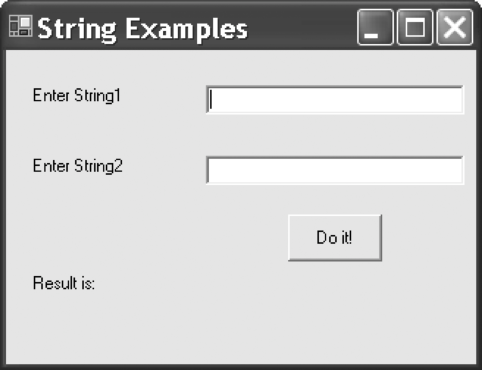
\includegraphics[width=8cm]{strings_example_screen}
			\caption{Screenshot of framework for string examples.}
			\label{fig:strings_example_screen}
		\end{figure}

		
	\section{Amending strings}
		Here we look at methods which change a string. Behind the scenes, these methods create a new string rather than changing the original string.

		\subsection*{\keyword{ToLower}}
			The \keyword{ToLower} method converts any upper-case letters in a string into lower-case letters, as in:
			\begin{lstlisting}
string1 = "Version 1.1"
resultString = string1.ToLower()
			\end{lstlisting}
			which puts \keyword{"version 1.1"} in \keyword{resultString}. You can experiment with this by using the following lines of code:
			\begin{lstlisting}
'code example:
string1 = String1Box.Text
ResultLabel.Text = string1.ToLower()
			\end{lstlisting}

		\subsection*{\keyword{ToUpper}}
			The \keyword{ToUpper} method does a similar operation as \keyword{ToLower}, but changes any lower-case letters into upper-case equivalents. For example:
			\begin{lstlisting}
string1 = "Basic"
resultString = string1.ToUpper()
			\end{lstlisting}
			would set \keyword{resultString} to "BASIC".

		\subsection*{\keyword{Trim}}
			The \keyword{Trim} method removes spaces from both ends of a string. If we put:
			\begin{lstlisting}
string1 = "     Center     "
resultString = string1.Trim()
			\end{lstlisting}
			then \keyword{resultString} becomes \keyword{"Center"}. Here is some code to exercise \keyword{Trim}:
			\begin{lstlisting}
'code example:
string1 = String1Box.Text
ResultLabel.Text = string1.Trim()
			\end{lstlisting}

		\subsection*{\keyword{Insert}}
			This method lets us insert characters into a string at a specified position, as in:
			\begin{lstlisting}
string1 = "Visual programming"
resultString = string1.Insert(7, "Basic ")
			\end{lstlisting}
			The result is \keyword{"Visual Basic programming"}. Here we inserted a string at character number 7 (\keyword{"p"}). The characters from \keyword{"p"} onwards are shifted right to make room. Here is some code to use:
			\begin{lstlisting}
'code example:
MessageBox.Show("Enter the string to insert, and position to put it")
string1 = String1Box.Text
n = CInt(String2Box.Text)
string2 = "A string to insert into ..."
ResultLabel.Text = string2.Insert(n, string1)
			\end{lstlisting}

		\subsection*{\keyword{Remove}}
			This method removes a given number of characters at a given position, as in:
			\begin{lstlisting}
string1 = "Deadline"
resultString = string1.Remove(1, 4)
			\end{lstlisting}
			The order of arguments is, first, the starting position, followed by the number to remove. The result is \keyword{"Dine"}, because 4 characters, starting at position 1 (the character \keyword{"e"}) have been removed. Here is some code to use:
			\begin{lstlisting}
'code example:
MessageBox.Show("Enter the start position, and 
 the number of characters to remove")
m = CInt(String1Box.Text)
n = CInt(String2Box.Text)
string1 = "An example string to remove from ..."
ResultLabel.Text = string1.Remove(m, n)
			\end{lstlisting}


	\section{Examining strings}
		These methods and properties allow us to examine a string - for example, to extract a section of it. A section of a string is often called a substring.

		\subsection*{\keyword{Length}}
			The \keyword{Length} property provides the number of characters in a string, as in:
			\begin{lstlisting}
string1 = "VB Programming"
resultString = CStr(string1.Length)
			\end{lstlisting}
			Here, n is set to 14.

		\subsection*{\keyword{Substring}}
			The \keyword{Substring} method copies a specified part of a string. We provide the starting position, and the number of characters to be copied. For example:
			\begin{lstlisting}
string1 = "position"
resultString = string1.Substring(2, 3)
			\end{lstlisting}
			We have selected from \keyword{s} (which is at index 2) for 3 characters, hence the result is \keyword{sit}. The value of \keyword{string1} is unchanged. 
			
			Here is the code for the example program, which displays its input with the first and last characters removed.
			\begin{lstlisting}
'code example:
MessageBox.Show("Enter the start position, and 
	the number of characters to copy")
m = CInt(String1Box.Text)
n = CInt(String2Box.Text)
string1 = "An example string to take a substring from"
ResultLabel.Text = string1.Substring(m, n)
			\end{lstlisting}
			A common use is to fetch a single character from a string, as in:
			\begin{lstlisting}
n = 3
string1 = string2.Substring(n)
		  \end{lstlisting}
			Varying \keyword{n} in a loop allows us to extract each character in turn.
			
		\begin{stqb}
			\begin{STQ}
			\item Explain the effect of the following code:
				\begin{lstlisting}
	Dim word As String = "possible"
	Dim s As String = word.Substring(1, word.Length-2)
				\end{lstlisting}
			\end{STQ}
		\end{stqb}

		\subsection*{\keyword{IndexOf}}
			This method determines whether a substring is contained within a string. We can also provide an offset, specifying where the search is to start. For example:
 			\begin{lstlisting}
string1 = "mississippi!"
n = string1.IndexOf("is")
			\end{lstlisting}
			sets \keyword{n} to 1, showing the position of the first \keyword{is}. (Recall that the first position of a string is numbered 0.)
			
			However, if we put:
			\begin{lstlisting}
string1 = "mississippi!"
n = string1.IndexOf("is", 3)
			\end{lstlisting}
			then \keyword{n} becomes 4, as the first occurrence is ignored. If the string is not found, −1 is returned.
			
			Here is some code for the example program, which reports on whether a string contains a substring.
			\begin{lstlisting}
'code example:
MessageBox.Show("Enter main string, then substring")
string1 = String1Box.Text
string2 = String2Box.Text
If string1.IndexOf(string2) = -1 Then
	ResultLabel.Text = "not found!"
Else
	ResultLabel.Text = "found"
End If
			\end{lstlisting}

		\subsection*{\keyword{IsNumeric}}
			Strictly, \keyword{IsNumeric} is a function, not part of the \keyword{String} class, but it is useful, and we cover it here for convenience. It returns a \keyword{Boolean} value indicating if its string argument is a valid number. Here is an example:
			\begin{lstlisting}
If IsNumeric(TextBox1.Text) = False Then
	MessageBox.Show("Error in number")
Else
	n = CInt(TextBox1.Text)
End If
			\end{lstlisting}

		\subsection*{\keyword{Split}}
			Here we are concerned with breaking a string up into sections. There is a method named \keyword{Split} in the \keyword{String} class, but it is not as simple to use as the \keyword{Split} function. Here is an example of the latter:
			\begin{lstlisting}
Dim words() As String
string1 = "Guitar, bass , drums"
words = Split(string1, ",")
For n = 0 To UBound(words)
	words(n) = words(n).Trim()
Next
			\end{lstlisting}
			Note that we do not use \keyword{Split} with a 'dot'. It is not a method of the \keyword{String} class. It is a function, and in fact existed in previous (non-object-oriented) versions of VB. We supply it with a string to split, and a string containing a separator character. Here, a comma is used as a separator between the three items, but we have made the data more realistic by adding extra spaces. The \keyword{Split} function returns an array of strings set to the appropriate size (which we don't know in advance of course). In the above example, you will see that the array of strings has been declared without a size, which is unusual, but is allowed. Later, we use it to hold the result from \keyword{Split}, and at this point we can use the \keyword{UBound} function to control a loop which processes each item in turn. Here, the processing involves trimming the extra spaces. Prior to trimming, the array values are:
			\begin{lstlisting}
"Guitar"
"  bass "
" drums"
			\end{lstlisting}
			After trimming, we have:
			\begin{lstlisting}
"Guitar"
"bass"
"drums"
			\end{lstlisting}

		\subsection*{\keyword{LastIndexOf}}
			This method is similar in concept to \keyword{IndexOf}, but returns the position of the rightmost occurrence of a substring. The value −1 is returned if no match is found. Here is an example:
			\begin{lstlisting}
string1 = "\directory\file"
n = string1.LastIndexOf("\")
			\end{lstlisting}
			The value 10 is returned.

		\subsection*{\keyword{StartsWith}}
			This method is used to find out if a string starts with a particular substring. It avoids the added complexity of using the \keyword{Length} property. The method returns a \keyword{Boolean} value. For example:
			\begin{lstlisting}
string1 = "http://path/page.html"
startsResult = string1.StartsWith("http")
			\end{lstlisting}
			would set \keyword{startsResult} to true.
			
			Here is some code for the example program, which determines whether a substring is present at the start of another string:
			\begin{lstlisting}
'code example:
MessageBox.Show("Enter main string, and string " &
		" to find at start")
string1 = String1Box.Text
string2 = String2Box.Text
If string1.StartsWith(string2) Then
	ResultLabel.Text = "Found at start!"
Else
	ResultLabel.Text = "Not found at start"
End If
			\end{lstlisting}

		\subsection*{\keyword{EndsWith}}
			This method is used to find out if a string ends with a particular substring. Yes, you could use a combination of other methods to accomplish this, but the provided method is less error-prone. The method returns a \keyword{Boolean} value. For example:
			\begin{lstlisting}
string1 = "http://path/page.html"
endsResult = string1.EndsWith("html")
			\end{lstlisting}
			would set \keyword{endsResult} to true.

			Here is some code for the example program, which determines whether a substring is present at the end of another string:
			\begin{lstlisting}
'code example:
MessageBox.Show("Enter main string, and string " &
		" to find at end")
string1 = String1Box.Text
string2 = String2Box.Text
If string1.EndsWith(string2) Then
	ResultLabel.Text = "Found at end!"
Else
	ResultLabel.Text = "Not found at end"
End If
			\end{lstlisting}
	

	\section{An example of string processing}
		Here we will look at the creation of a string processing method which performs a commonly required task - to examine a string, replacing every occurrence of a given substring by another substring (of potentially different length). Note that the \keyword{String} class has a \keyword{Replace} method, but it can only replace a single character. Closer to home, there is a \keyword{Replace} function (not a member of the \keyword{String} class) which does what we require. However, it is instructive to look at the programming of such a method. We shall name it \keyword{Change} to avoid any conflict with the existing \keyword{Replace} function.
		
		Here is an example of changing substrings. If we have the string:
		\begin{lstlisting}
"to be or not to be"
		\end{lstlisting}
		and we replace every occurrence of \keyword{"be"} with \keyword{"eat"}, we will create:
		\begin{lstlisting}
"to eat or not to eat"
		\end{lstlisting}
		The basic process is to use \keyword{IndexOf} to determine the position of a substring - \keyword{"be"} here. We then form a new string made up of the left part of the string, the right part, and the replacement string in the centre. We have:
		\begin{lstlisting}
"to " & "eat" & " or not to be"
		\end{lstlisting}
		The process must then be repeated until there are no more occurrences of \keyword{"be"}. There are three problem cases:
		\begin{itemize}
			\item The user of \keyword{Change} asks us to replace a value of \keyword{""}. We could regard any string as being preceded by an infinite number of such empty strings! Our approach here is to simply return the unchanged original string.
			\item The replacement string contains the string to be replaced. For example, we might try to change \keyword{"be"} to \keyword{"beat"}. To prevent an infinite number of replacements taking place, we ensure that we only consider substrings in the right-hand part of the string. We use the variable \keyword{startSearch} to keep track of the start of the right-hand part of the string.
			\item The replacement string combined with the original string produces the string to be replaced. For example, when we replace \keyword{bc} with \keyword{c} in \keyword{abbcd}, we get \keyword{abcd}. The solution to the previous case also handles this possibility.
		\end{itemize}
		The full code is:
		\begin{lstlisting}
Private Function Change(original As String,
					fromText As String,
					toText As String) As String
	Dim leftBit, rightBit As String
	Dim startSearch As Integer = 0
	Dim place As Integer = original.IndexOf(fromText)
	If fromText.Length <> 0 Then
		While place = startSearch
			leftBit = original.Substring(0, place)
			rightBit = original.Substring(
				place + fromText.Length,
				original.Length - place - fromText.Length)
			MessageBox.Show(leftBit)
			MessageBox.Show(rightBit)
			original = leftBit & toText & rightBit
			startSearch = leftBit.Length + toText.Length
			place = original.IndexOf(fromText)
		End While
	End If
	Return original
End Function
		\end{lstlisting}
		Here is how we might use our method:
		\begin{lstlisting}
Dim original As String = "to be or not to be"
Dim changed As String = Change(original, "be", "eat")
		\end{lstlisting}
		Now we will incorporate it into a program.


	\section{Case study - Ask Frasier}
		In 1970, Joseph Weizenbaum wrote a program known as ELIZA to simulate a particular style of psychiatrist. It was a simple program, in the sense that it made little attempt to understand the sense of the input that users (patients) typed. For example, if the patient entered:
		\begin{lstlisting}
I am feeling sad
		\end{lstlisting}
		then ELIZA might respond with:
		\begin{lstlisting}
you are feeling sad - why?
		\end{lstlisting}
		Similarly, if the patient typed:
		\begin{lstlisting}
I am feeling VB
		\end{lstlisting}
		then ELIZA might respond with:
		\begin{lstlisting}
You are feeling VB - why?
		\end{lstlisting}
		\begin{figure}[bth]
			\centering
			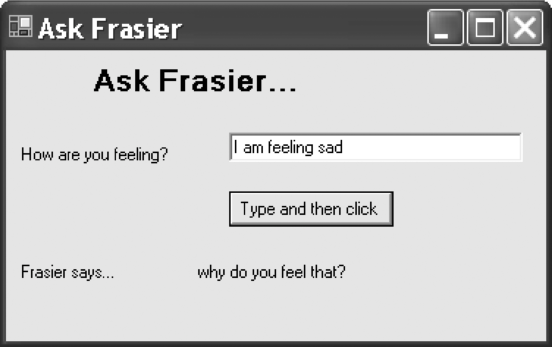
\includegraphics[width=10cm]{strings_frasier_screen}
			\caption{Screenshot of framework for string examples.}
			\label{fig:strings_frasier_screen}
		\end{figure}
		Here we present an even more simplified version, which we will call Ask Frasier, after the US sitcom character. Basically, we will write a method named \keyword{GetReply}, which has a question as its argument, and which returns a reply. The input string comes from a textbox, and the reply is displayed in a label. \Vref{fig:strings_frasier_screen} shows a screenshot, and here is the code:
		\begin{lstlisting}
Private Sub Button1_Click(
			sender As System.Object,
			e As System.EventArgs)
			Handles Button1.Click
	ReplyLabel.Text = getReply(QuestionBox.Text)
End Sub
Private Function getReply(question As String)
				As String
	Dim randomNumber As Random = New Random()
	Dim variation As Integer
	Dim reply As String
	question = " " & question & " "
	variation = randomNumber.Next(0, 2)
	If variation = 0 Then
		reply = transform(question)
	ElseIf variation = 1 Then
		reply = "why do you feel that?"
	Else
		reply = "Please be frank!"
	End If
	Return reply
End Function
Private Function transform(question As String)
				As String
	Dim tempReply As String		
	If question.IndexOf(" I ") >= 0 Then
		tempReply = Change(question, " I ", " you ")
		tempReply = Change(tempReply, " am ", " are ")
		Return Change(tempReply, " my ", " your ") &
					"-why?"
	ElseIf question.IndexOf(" no ") >= 0 Then
		Return "'no'? - that is negative! Please explain."
	Else
		Return "'" & question & "' -Please explain."
	End If
End Function
		\end{lstlisting}
		Note that we must paste in the code for our \keyword{Change} method.
		
		To make the responses seem more human, we add an element of randomness:
		\begin{lstlisting}
variation = randomNumber.Next(0, 2)
If variation = 0 Then
	reply = transform(question)
ElseIf variation = 1 Then
	reply = "why do you feel that?"
Else
	reply = "Please be frank!"
End If
		\end{lstlisting}
		The random integer provides three cases. In two of them, we produce a standard reply, but in the other case, we transform the question, by e.g. replacing every \keyword{" I "} with \keyword{" you "}. We add extra spaces at the start and end of the question to assist in detecting whole words. Note that the program has no knowledge of English meanings or grammar. To add this would involve a major programming effort.


	\section{Programming principles}
		\begin{itemize}
      \item A string contains a sequence of characters.
      \item Strings can be operated on by methods, and with the relational operators.
		\end{itemize}


	\section{Programming pitfalls}
	\begin{itemize}
      \item Strings are objects, and the \keyword{String} class provides methods and properties. 
				The correct usage for its methods is, for example:
				\begin{lstlisting}
n = string1.IndexOf("/")
				\end{lstlisting}
				rather than:
				\begin{lstlisting}
n = IndexOf(string1)
				\end{lstlisting}
      \item The exceptions to this are \keyword{Length}, which is a property and has no brackets, and \keyword{Split} and \keyword{IsNumeric}, which are functions, not part of the class \keyword{String}.
	\end{itemize}


	\section{Grammar spot}
		The \keyword{String} class methods require us to provide a string to be operated on, as in:
		\begin{lstlisting}
Dim s As String = "demo"
n = s.Length
		\end{lstlisting}
		Note that we can supply a literal string, or a method call which returns a string, as in:
		\begin{lstlisting}
n = "another demo".Length
n = s.Substring(0, 2).Length ' length of "de"
		\end{lstlisting}

		
	\section{New language elements}
		The use of \keyword{""} within quoted strings, to stand for a single quote.


	\section{New IDE facilities}
		No new IDE facilities are introduced in this chapter.


	\section{Summary}
		\begin{itemize}
      \item Instances of the class \keyword{String} contain a sequence of characters. The first character is at position 0.
      \item \keyword{String} instances can be declared and created by e.g.:
		\begin{lstlisting}
Dim s As String
Dim name As String = "Mike"
		\end{lstlisting}
      \item The most useful facilities for string manipulation are: 
				
				\begin{itemize}
					\item the use of relational operators(\keyword{>}, etc.) to determine the order of strings.
					\item	Amending strings:	
						
						\begin{tabular}{>{\collectcell\keyword}l<{\endcollectcell} }
							ToUpper\\
							ToLower \\
							Trim\\
							Insert\\
							Remove
						\end{tabular}

					\item	Examining strings: 
						
						\begin{tabular}{>{\collectcell\keyword}l<{\endcollectcell} }
							Length\\
							Substring \\
							IndexOf\\
							LastIndexOf\\
							StartsWith\\
							EndsWith\\
							IsNumeric \\
							Split
						\end{tabular}
		
					\item	Conversion:
		
						\begin{tabular}{>{\collectcell\keyword}l<{\endcollectcell} }
							CStr\\
							CInt \\
							CDbl\\
						\end{tabular}
				\end{itemize}
		\end{itemize}


	\section{Exercises}
		\begin{EXE}
			\item	Write a program which inputs two strings from text boxes, and which joins them together. Show the resulting string and its length in labels.
			\item	Write a program which inputs one string and determines whether or not it is a palindrome. A palindrome reads the same backwards and forwards, so 'abba'is a palindrome. Assume that the string contains no spaces or punctuation.
			\item	Write a program to input a string which can be an \keyword{Integer} or a \keyword{Double} number in a textbox. Display the type of the number. Assume that a \keyword{Double} contains a decimal point.
			\item Modify the Ask Frasier program to make it more human, by adding more variation to the replies.
			\item	\label{it:string_input} Write a program which allows input of the form:
				\begin{lstlisting}
123 + 45
6783 - 5
				\end{lstlisting}
				(i.e. two integers with + or - between them, and with spaces separating items) and which displays the result of the calculation.
			\item Extend Exercise \ref{it:string_input} so that input of the form:
				\begin{lstlisting}
12 + 345 − 44 − 23 − 57 + 2345
				\end{lstlisting}
				can be handled. Assume that the user will make no errors.
				(Hint: the pattern of such input is an initial number, followed by any number of operator/number pairs. Your program should handle the initial number, then loop to handle the following pairs.)
			\item Extend Exercise \ref{it:string_input} so that input can take two forms:
				\begin{lstlisting}
setm 2 426
12 + m2
				\end{lstlisting}

				The \keyword{setm} instruction is followed by two numbers. The first one refers to a memory store numbered from 0 to 9, and the second one is a number which is to be stored in the memory. Calculations can now be done using integers as earlier, and also memory names. (Hint: use an integer array to represent the memory.) Extend your program so that the following forms are processed: 
				\begin{lstlisting}
m3 = 12 + m5 - 328 - m7
display m3
				\end{lstlisting}

			\item	Write a program which inputs a suggested email address, and reports on whether it should be allowed or not. The address must be of the form:
				\begin{lstlisting}
somename@some.address
				\end{lstlisting}
				It must not contain spaces or other punctuation. Finally, extend the program so it rejects addresses which have special words in them, such as 'webmaster', 'government', etc. These special words are to be set up in a list box by the user.
		\end{EXE}

		\begin{stab}*
			\begin{enumChapter}
				\item We extract everything but the first and last character, so \keyword{s} becomes \keyword{"ossibl"}.
			\end{enumChapter}
		\end{stab}

